\documentclass[12pt]{article}
\usepackage[T1]{fontenc}
\usepackage{calc}
\usepackage{setspace}
\usepackage{multicol}
\usepackage{fancyheadings}

\usepackage{graphicx}
\usepackage{color}
\usepackage{rotating}
\usepackage{harvard}
\usepackage{aer}
\usepackage{aertt}
\usepackage{verbatim}

\setlength{\voffset}{0in}
\setlength{\topmargin}{0pt}
\setlength{\hoffset}{0pt}
\setlength{\oddsidemargin}{0pt}
\setlength{\headheight}{0pt}
\setlength{\headsep}{.4in}
\setlength{\marginparsep}{0pt}
\setlength{\marginparwidth}{0pt}
\setlength{\marginparpush}{0pt}
\setlength{\footskip}{.1in}
\setlength{\textwidth}{6.5in}
\setlength{\textheight}{9in}
\setlength{\parskip}{0pc}

\renewcommand{\baselinestretch}{1.4}

\newcommand{\bi}{\begin{itemize}}
\newcommand{\ei}{\end{itemize}}
\newcommand{\be}{\begin{enumerate}}
\newcommand{\ee}{\end{enumerate}}
\newcommand{\bd}{\begin{description}}
\newcommand{\ed}{\end{description}}
\newcommand{\prbf}[1]{\textbf{#1}}
\newcommand{\prit}[1]{\textit{#1}}
\newcommand{\beq}{\begin{equation}}
\newcommand{\eeq}{\end{equation}}
\newcommand{\bdm}{\begin{displaymath}}
\newcommand{\edm}{\end{displaymath}}
\newcommand{\script}[1]{\begin{cal}#1\end{cal}}
\newcommand{\citee}[1]{\citename{#1} (\citeyear{#1})}
\newcommand{\h}[1]{\hat{#1}}
\newcommand{\ds}{\displaystyle}

\newcommand{\app}
{
\appendix
}

\newcommand{\appsection}[1]
{
\let\oldthesection\thesection
\renewcommand{\thesection}{Appendix \oldthesection}
\section{#1}\let\thesection\oldthesection
\renewcommand{\theequation}{\thesection\arabic{equation}}
\setcounter{equation}{0}
}

\pagestyle{fancyplain}
\lhead{}
\chead{Regime Switching, Learning, and the Great Moderation}
\rhead{\thepage}
\lfoot{}
\cfoot{}
\rfoot{}

\begin{document}

\begin{titlepage}
\begin{singlespace}
\title{Regime Switching, Learning, and the Great Moderation\footnote{This is very preliminary and very incomplete.  I am grateful for the advice and guidance of Eric Leeper, Kim Huynh, Brian Peterson, and Todd Walker; for useful conversations with Fabio Milani and Bruce Preston; and for comments by the participants of Indiana University economics department seminars.  All errors are my own.}}
\date{\today}
\author{James Murray\\
Department of Economics\\
Indiana University\footnote{\textit{Mailing address}: 100 S Woodlawn, Bloomington, IN  47405. \textit{E-mail address}: jmmurray@indiana.edu.  \textit{Phone number}: (574)315-0459. }}

\maketitle

\thispagestyle{empty}

\abstract{This paper examines empirically how the ``bad luck'' explanation can explain changing volatility in U.S. inflation and output when agents do not have rational expectations, but instead form expectations with least squares learning with an endogenously changing learning gain.  Bad luck is modeled into a standard New Keynesian model by augmenting it with two states that evolve according to a Markov chain, where one state is characterized by large variances for structural shocks, and the other state has relatively smaller variances.  Agents in a model are completely unaware of the state changing process and the underlying parameters of the model and instead form expectations by computing least squares regressions.  Agents do suspect, however, that structural changes may occur, and so endogenously decide how much weight to give data further in the past based on the size of recent forecast errors relative to the average size of forecast errors.  This type of endogenously changing learning mechanism can create periods of excess volatility without the need for changes in the variance of the underlying shocks.  Therefore, when taking this model to the data, the degree of bad luck needed to explain volatile periods in U.S. history may not be as great as when assuming rational expectations or learning with a constant gain.} \newline 

\noindent \textit{Keywords}: Learning, regime switching, great moderation, New Keynesian model, maximum likelihood. \\
\noindent \textit{JEL classification}: C13, E31, E50.
\end{singlespace}
\end{titlepage}

\newpage
\section{Introduction}
Figure \ref{fg:data} shows plots of the growth rate of real GDP and the GDP deflator annualized inflation rate for the United States since 1957.  Aside from business cycle fluctuations, the data is characterized by changing periods of volatility.  Macroeconomics has had difficulty explaining what has become to be called the Great Moderation, the period of excessive volatile during the late 1970s and early 1980s, followed by a relatively moderate period since the mid-1980s.  This paper is also concerned with explaining the relatively moderate period during the 1960s, despite receiving less attention in the literature.

Leading explanations for these changes in volatility can be described as, good vs. bad policy, and good vs. bad luck.  \citee{ls2004} find empirical evidence of a change in monetary policy from bad to good, occurring sometime between 1979 and 1982.  They find that prior to 1979, monetary policy did not adjust the federal funds rate by more than one-to-one with inflation, and therefore under rational expectations, the equilibrium was indeterminate and the economy was subject to sunspot shocks which would lead to greater volatility.  \citee{milani2005} estimates a similar model, but instead assumes that agents are not rational, but form expectations according to least squares learning.  When splitting the sample at the same dates as \citee{ls2004}, he finds little evidence of a change in monetary policy, finding the federal funds rate did adjust by more than one-to-one with inflation throughout the sample.  

\citee{primiceri2005} incorporates learning and finds evidence of bad vs. good policy in an empirically founded model of unemployment rate and inflation determination.  The ``bad'' policy in this work is actually characterized by optimal behavior by the central bank during the 1970s, but mis-perceptions by the central bank of the natural rate of unemployment and the degree of persistence of inflation lead to the wrong policy prescription.  As time progresses and the central bank collects more data, it learns its mistake and eventually provides better policy, leading to period of great moderation.

\citee{simszha2006} examine whether changes in U.S. volatility came from changes in luck or changes in policy by using a structural VAR with regime switching that only makes restrictions for identifying monetary policy, but otherwise leaves the model free of restrictions to allow for any interpretation of consumer and producer behavior.  They find that the best fitting model is one with only bad luck.  That is, the model that allows for no regime change in policy or behavior, and only regime change in the variances of structural shocks.

In this paper, I examine a version of the ``bad luck'' story in the framework of a New Keynesian model where agents do not capable of rational expectations, but instead form expectations by running least squares regressions.  I assume a simple model with only two states, one characterized by large variances for the structural shocks, and one characterized by relatively smaller variances.  I assume the state evolves according to Markov chain were the current state is only dependent on the previous state, and the probabilities of switching between states is exogenous.  

I assume agents do not have rational expectations, and are therefore completely unaware that there are two states of the economy, and that these states follow a Markov chain switching process.  Agents do, however, remain suspect that structural changes may occur.  They do have any knowledge about what types of structural changes are possible, or any idea with what probabilities structural changes can occur.  I assume that expectations evolve according to the \citee{marcetnicolini2003} framework where the weight agents give observations that occurred further into the past is endogenous.  Specifically, agents begin using a decreasing learning gain which consistent with ordinary least squares and no suspicion of structural change.  However, if recent forecast errors become larger than the historical average, agents then suspect a structural change may have occurred and therefore increase their learning gain, giving larger weight to current observations which are believed to occur after a structural shock.

While a constant learning gain is theoretically capable of producing time varying volatility, in \citee{murray2007} I show in a New Keynesian model with no regime changes that constant gain learning is not able to deliver dynamics of U.S. inflation and output much better than rational expectations, and both frameworks especially fail to explain the excess volatility of the 1970s.  \citee{milani2007} simulates a model estimated with U.S. data that includes the endogenously changing learning gain suggested by \citee{marcetnicolini2003} and finds that this type of learning can effectively explain significant changes in volatility.  Moreover, his estimates imply that during most of the 1970s decade, agents suspected structural change and therefore used a high constant gain.  

This paper builds on Milani's analysis by also allowing for recurrent regime changes in the volatility of the structural shock.  Estimation of this model will decompose of the explanation for changes in volatility into changes in the volatility of structural shocks, and endogenous changing in the learning gain.  Since both of these mechanisms deliver greater volatility, I expect the results to indicate that periods of excessive volatility are explained by a mixture of changes in learning and changes in luck.  Furthermore, I expect that when failing to allow for changes in the learning gain one will over estimate both the frequency of the ``bad'' regime occurring, and the volatility of the shocks that occur during the bad regime.

\section{Model}
The crucial extentions of an endogenously changing learning gain and a Markov chain process for changes in structural volatility are incorporated into a standard New Keynesian model of output and inflation determination and monetary policy.  There are a continuum of consumers types on the unit interval, and a continuum of intermediate goods producers on the same unit interval.  Each consumer type as a specific labor skill that is only hired by the corresponding intermediate goods producer.  It is assumed there are a number of consumers of each type, so that no consumer has market power over the wage, and that there are an equal number of consumers in each type, so that relative output levels of intermediate goods do not depend on the distribution of consumer types.

There is one final good that is used for consumption, and produced using all the intermediate goods.  The intermediate goods are imperfect substitutes for eachother in production, therefore intermate goods firms are monopolistically competitive.  Prices for intermediate goods are subject to a \citee{calvo1983} pricing friction where only a fraction of firms are able to re-optimize their price every period, and the firms fortunate to do so is randomly determined, independently of firms' histories.

\subsection{Consumers}
Each consumer type has a specific labor skill that can only be hired by a specific intermediate goods producing firm.  Since each intermediate goods firm has a different labor demand, wage income will be different for each consumer type.  Given a perfect asset market, though, consumption will be equal across all consumers.  Each consumer type $i \in (0,1)$ maximizes utility,
\bdm E_0^* \sum_{t=0}^{\infty} \beta^t \left[ \frac{1}{1-\frac{1}{\sigma}} \xi_t \left(c_t - \eta c_{t-1}\right)^{1-\frac{1}{\sigma}} - \frac{1}{1+\frac{1}{\mu}} n_t(i)^{1+\frac{1}{\mu}} \right], \edm
subject to the budget constraint,
\bdm c_t + b_t(i) = \frac{1+r_{t-1}}{1+\pi_t} b_{t-1}(i) + \frac{w_t(i)}{p_t} n_t(i) + \Pi_t - \tau_t \edm
where the expectation operator $E_t^*$ denotes possibly non-rational expectations.  Consumption at time $t$, given by $c_t$, is not indexed by individual type $i$ since it is equal across all agents.  The remaining variables include $\xi_t$ which is an aggregate preference shock, $n_t(i)$ and $w_t(i)/p_t$ are the labor supply and real wage of individual $i$ at time $t$, respectively, $b_t(i)$ is individual $i$'s purchase of real government bonds at time $t$, $r_t$ is the nominal interest rate paid on government bonds, $\pi_t$ is the inflation rate of the price of the final good, $\Pi_t$ is the value of profits earned by owning stock in firms, and $\tau_t$ is the value of real lump sum taxes.  The preference parameters are $\sigma \in (0,\infty)$, which is the intertemporal elasticity of substitution, $\mu \in (0,\infty)$ which is the elasticity of labor supply, and $\eta \in [0,1)$, which is the degree of habit formation.  

Habit formation is added to the model because it introduces a source of consumption (and therefore output) persistence that has been found to be significant in rational expectations models.  For example \citee{smetswouters2005} estimate a rational expectations New Keynesian model with numerous for both the United States and Euro area and find point estimates for the degree of habit formation very close to 1.  Furthermore, \citee{fuhrer2000} finds that habit formation leads to ``hump shaped'' impulse response functions that can be supported by the data.  The importance of habit formation may not be so important when dropping the assumption of rational expectations.  \citee{milani2005} estimates a New Keynesian model with learning, and shows that under learning, the degree of habit formation falls close to zero.

Log-linearizing the consumers' first order conditions leads to the following Euler equation,
\beq \label{eq:lneuler} \h{\lambda}_{t} = E_t^* \h{\lambda}_{t+1} + \h{r}_t - E_t^* \pi_{t+1}, \eeq
where a hat indicates the percentage deviation of the variable from its steady state.\footnote{A hat is omitted from inflation because it will be necessary to assume the steady state inflation rate is equal to zero when log-linearizing the firms' profit maximizing conditions.}  Here, $\h{\lambda}_t$ is the marginal utility of real income, given by,
\beq \label{eq:lnlambda} \h{\lambda}_t = \frac{1}{ (1-\beta \eta)(1-\eta)}\left[ \beta \eta \sigma E_t^* \h{c}_{t+1} - \sigma(1+\beta \eta^2) \h{c}_t + \sigma \eta \h{c}_{t-1} \right] + \left(\h{\xi}_t - \beta \eta E_t^* \h{\xi}_{t+1} \right). \eeq

\subsection{Production}
There is one final good used for consumption and investment which is sold in a perfectly competitive market and produced with a continuum of intermediate goods.  The production function is given by,
\beq \label{eq:yprod} y_t = \left[ \int_0^1 y_t(i)^{\frac{\theta-1}{\theta}} di \right]^{\frac{\theta}{\theta-1}}, \eeq
where $y_t$ is the output of the final good, $y_t(i)$ is intermediate good $i$, and $\theta \in (1,\infty)$ is the elasticity of substitution in production.  Profit maximization leads to the demand for each intermediate good,
\beq \label{eq:yi} y_t(i) = \left[ \frac{p_t(i)}{p_t} \right]^{-\theta} y_t, \eeq
where $p_t(i)$ is the price of intermediate good $i$ and $p_t$ is the price of the final good.  Substituting equation (\ref{eq:yi}) into (\ref{eq:yprod}) leads to a consumption price index that holds in equilibrium,
\beq \label{eq:pfinal} p_t = \left[ \int_0^1 p_t(i)^{1-\theta} di \right]^{\frac{1}{1-\theta}}. \eeq

Each intermediate good is produced according the constant returns to scale production function $y_t(i) = z_t n_t(i)$, where $z_t$ is an exogenous technology shock common to all firms.  Given a level of production $y_t(i)$, firms choose labor demand to minimize total cost $\frac{w_t(i)}{p_t}n_t(i)$.  When labor markets clear, it can be shown that firm $i$'s optimal choice for labor leads to the log-linearized marginal cost of firm $i$ equal to,
\beq \label{eq:mc} \h{\psi}_t(i) = \frac{1}{\mu} \h{y}_t(i) - \h{\lambda}_t - \left(\frac{1}{\mu} + 1\right) \h{z}_t. \eeq
Summing equation (\ref{eq:mc}) across all firms leads to the average marginal cost in the economy,
\beq \label{eq:mc2} \h{\psi}_t = \frac{1}{\mu} \h{y}_t - \h{\lambda}_t - \left(\frac{1}{\mu} + 1\right) \h{z}_t. \eeq

Firms' pricing decisions are subject to the \citee{calvo1983} pricing friction, where only a constant fraction of firms are able to re-optimize their in a given period.  I suppose that firms who are not able to re-optimize their price may adjust their price by a fraction, $\gamma$, of the previous period's inflation rate.  Let $\omega \in (0,1)$ denote the fraction of firms who are not able to re-optimize their prices each period.  Since these specific firms are randomly determined, $\omega^T$ is the probability a firm will not be able to re-optimize its price for $T$ consecutive periods.  A firm who is able to re-optimize its price maximizes the following present discounted utility value of profits earned while the firm is unable to re-optimize its price again:
\beq \label{eq:intprofit}
E_t^* \sum_{T=0}^{\infty} \left(\omega \beta \right)^{T} \frac{\lambda_{t+T}}{\lambda_t}
\left\{ \left(\frac{p_{t}(i) \pi_{t+T}^{*}}{p_{t+T}}\right) y_{t+T}(i) - \Psi\left[y_{t+T}(i)\right] \right\},
\eeq
where $\Psi\left[y_{t+T}(i)\right]$ is the real total cost function of producing $y_{t+T}(i)$ units, given the optimal decision for labor, and $\pi_{t+T}^{*} = \prod_{j=1}^{T} (1+\gamma \pi_{t+j-1})$ is degree to which the firm's price is able to be adjusted according to inflation indexation.  It can be shown that the first order condition for $p_{t}(i)$ combined with the final good price index, equation (\ref{eq:pfinal}), leads to the log-linear Phillips equation,
\beq \label{eq:phillips} \pi_t = \frac{\gamma}{1+\beta \gamma} \pi_{t-1} + \frac{\beta}{1+\beta\gamma} E_t^* \pi_{t+1} + \frac{(1-\omega)(1-\omega \beta)}{\omega (1+\theta \mu) (1+\beta \gamma)} \h{\psi}_t \eeq

\subsection{Monetary Policy}
The nominal interest rate is determined jointly with output and inflation by monetary policy.  In this paper I assume the monetary authority follows a \citee{taylor1993} type rule of the form,
\beq \label{eq:taylor} \h{r}_t = \rho_r \h{r}_{t-1} + (1-\rho_r) \left(\psi_{\pi} \pi_t + \psi_y \h{y}_t \right) + \epsilon_{r,t} \eeq
where $\rho_r \in [0,1)$ is a degree of interest rate smoothing desired by the monetary authority, $\psi_{\pi} \in (0,\infty)$ is the feedback on the interest rate to inflation, $\psi_y \in (0,\infty)$ is the feedback on the interest rate to deviations of output from the steady state, and $\epsilon_{r,t}$ is an independently and identically distributed exogenous monetary policy shock.

\subsection{Regime Switching}
The bad luck explanation for why the United States experienced periods of excessive volatility is that the variances of the structural shocks were larger during these periods.  To model this explanation in the framework of the New Keynesian model I suppose the variance of the technology shock, $z_t$, and the preference shock, $\xi_t$, are determined by two states.  Let state 1, denoted by $s_1$, be the state where the shocks are relatively less volatile, and state 2, denoted by $s_2$, be the state where the shocks are relatively more volatile.  I furthermore assume that these shocks may be serially correlated, so they evolve according to,
\beq z_t = \rho_z z_{t-1} + \epsilon_{z,t}(s_t) \eeq
\beq \xi_t = \rho_{\xi} \xi_{t-1} + \epsilon_{\xi,t}(s_t) \eeq
where the innovation of the shocks depend on the state.  The innovations in a given state will be independently normally distributed with mean zero and variances given by,
\beq \label{eq:vars}
Var\left( \left[ \begin{array}{c} \epsilon_{z,t}(s_t) \\ \epsilon_{\xi,t}(s_t) \end{array} \right] \right) = \left\{
 \begin{array}{c} \left[ \begin{array}{cc} \sigma_{z,1}^2 & 0 \\ 0 & \sigma_{\xi,1}^2 \end{array} \right], \mbox{       if $s_t=1$} \\ 
\left[ \begin{array}{cc} \sigma_{z,2}^2 & 0 \\ 0 & \sigma_{\xi,2}^2 \end{array} \right], \mbox{       if $s_t=2$} \\
\end{array} \right \eeq

The state $s_t$ evolves according to a two state Markov chain.  Let $p_j \in (0,1)$ denote the probability of staying in state $j$ at time $t$, given the economy is at state $j$ at time $t-1$, for $j \in \{1,2\}$.  This implies that the probability of moving from state $j$ in $t-1$ to the other state in time $t$ is given by $1-p_j$ .  The state then evolves according to the transition matrix,
\beq \label{eq:tran} P = \left[ \begin{array}{cc} p_1 & 1-p_1 \\ 1-p_2 & p_2 \end{array} \right]. \eeq

\section{Learning}
I deviate from the rational expectations assumption and assume agents form expectations by computing least squares regressions and using these forecasts as their expectations.  I also assume that agents have no knowledge of the regime switching process and no knowledge about what types of regimes are possible or with what probabilities.  I do allow agents to adjust their expectations if they suspect structural changes have occurred.  One way to model this is to use constant gain learning, which is consistent with  agents' forecasts based on weighted least squares, where the weights decline geometrically with the age of the observations.  With a constant gain, the weight put on the latest observation is always the same, regardless of how much data the agents already have for their forecasts.  One benefit of this type of learning is that learning dynamics persist in the long run.  If agents instead use ordinary least squares (OLS), then the weight agents give to additional observations diminishes as their sample size approaches infinity.  Said another way, the learning gain decreases and approaches zero as time approaches infinity.  Learning dynamics therefore disappear completely in the long run when expectations are formed with OLS.

Authors such as \citee{sargent1999} and \citee{evanshonka2001} have suggested constant gain learning is a natural way to model agents which have a constant suspicion that their may have been a structural change.  Therefore every period agents give the most weight to the latest observations, and give lesser weight the longer ago an observation occurred.  Constant gain learning can in theory lead to time varying volatility of expectations, and therefore time varying volatility of outcomes for inflation and output.  This affect depends on the size of the constant gain, and for empirically plausible values, this type of learning fails to deliver very big effects.   \citee{williams2003} finds this to be the case in a simple model with simulated data.  In \citee{murray2007}, I show in an esimated New Keynesian model that constant gain learning provides dynamics very similar to rational expectations. 

\citee{marcetnicolini2003} suggest an alternative way to model dynamic expectations.  Instead of assuming that agents never suspect a structural change, as is consistent with OLS, or assuming that agents always suspect a structural change with equal likelihood, as is consistent with a constant gain, they take a mixture of these methods where the learning gain changes endogenously.  Suppose agents begin with no suspicion of structural change.  As time progresses they form their expectations using a decreasing learning gain consistent with OLS.  Agents then begin to suspect a structural change if recent forecast errors are larger than historical averages.  When this happens, agents switch to a relatively large learning gain.  As long as forecast errors are large, the learning gain remains at this high point.  When forecast errors start becoming small, the learning gain then starts decreasing from this high point at a rate consistent with OLS.  I explain explicitly this endogenous gain algorithm below, but first it is first necessary to explain, specific details of least squares learning in the framework of a dynamic stochastic general equilibrium model like the New Keynesian model in Section 2.

\subsection{Least Squares Learning}
The log-linearized model in Section 2 can be expressed in the general form:
\beq \label{eq:sform} \Omega_{0} x_t = \Omega_{1} x_{t-1} + \Omega_{2} E_t^* x_{t+1} + \Psi \epsilon_t(s_t), \eeq
where $x_t$ is a vector of minimum state variables (expressed in terms of percentage deviations form the steady state), all observable to agents in the model, and $\epsilon_t$ is a vector of structural shocks, which as discussed in the previous section, may be state dependent.  For the New Keynesian model examined in this paper $x_t = [\h{y}_t~ \pi_t~ \h{r}_t~ \h{z}_t~ \h{\xi}_t]'$, and $\epsilon_t(s_t) = [\epsilon_{z,t}(s_t)~ \epsilon_{\xi,t}(s_t)~ \epsilon_{r,t}]'$.  The minimum state variable solution of the model implies the rational expectation for $x_{t+1}$ is given by,
\beq \label{eq:msvsol} E_t x_{t+1} = G x_{t}, \eeq
where the elements of the matrix $G$ are a function of the parameters of the model and may be determined by the method of undetermined coefficients.\footnote{Log-linearizing the model eliminates any importance agents place on risk that is inherent in a non-linear solution of the model.  Equation (\ref{eq:msvsol}) is determined in a linear model and so is completely independent of the variance of the structural shocks.  In the non-linear model, risk may play an important role in agents behavior especially in the framework of regime switching volatility, but I ignore this avenue and suppose that changes in agents behavior not explained by the first order properties come from changes in expectations due to learning.}  Agents that form expectations by learning do not know any of the structural parameters and instead estimate the matrix $G$ by least squares.  

The timing in a given period of how agents make expectations and decisions is as follows.  At the begining of period $t$ agents wake up with data realized through period $t-1$.  They collect this data and use their least squares results to form an estimate for $G$ which they then use to make forecasts for future realizations of variables such as output and inflation.  Given these expectations, agents consumption and pricing decisions are implemented, and only then do time $t$ outcomes become realized.  In the next period, these outcomes are then available as data to the agents, and the process begins again.  

There is no constant term in the general form of the model, equation (\ref{eq:sform}), or in the rational expectation, given in equation (\ref{eq:msvsol}), since all variables are expressed in terms of percentage deviations from the steady state.  Since agents are not endowed with information about the parameters of the model, it is realistic to suppose that agents do not know steady state values.  Therefore, I suppose that agents also estimate a constant term in equation (\ref{eq:msvsol}).  Let $\h{G}_t^*$ denote agents' time $t$ estimate for matrix $G$ which also includes a column for a constant term so that.  Therefore, $\h{G}_t^* = [\h{g}_{0,t}~ \h{G}_t]$, where $\h{g}_{0,t}$ is the time $t$ estimate of the constant term and $\h{G}_t$ is the time $t$ estimate for $G$. 

If agents use OLS, then,
\beq \label{eq:Gsum} \left(\hat{G}_t^*\right)' = \left( \frac{1}{t-1} \sum_{\tau=1}^{t-1} x_{\tau-1}^* {x_{\tau-1}^{*}}' \right)^{-1} \left( \frac{1}{t-1} \sum_{\tau=1}^{t-1} x_{\tau-1}^* x_{\tau}' \right), \eeq 
where $x_t^* = [1~ x_t']'$ is the vector of regressors agents use, which is simply $x_t$ with a 1 augmented in order to estimate the constant term.   Agents then form the expectation,
\beq \label{eq:agfore} E_t^* x_{t+1} = \h{g}_{0,t} + \h{G}_t E_t^* x_t = (I + \h{G}_t)\h{g}_{0,t} + \h{G}_t^2 x_{t-1}. \eeq
The least squares estimate for $G_t^*$ can be rewritten as the following recursive form:
\beq \label{eq:lnG} \hat{G}_t^* = \hat{G}_{t-1}^* + g_t (x_{t-1} - \hat{G}_{t-1}^* x_{t-2}^*) {x_{t-2}^*}' R_t^{-1} ,\eeq
\beq \label{eq:lnR} R_t = R_{t-1} + g_t (x_{t-2}^* {x_{t-2}^*}' - R_{t-1}), \eeq
where $g_t=1/(t-1)$ is the learning gain.\footnote{To show this, let $R_t = \frac{1}{t-1} \sum_{\tau=1}^{t-1} x_{\tau-1}^* x_{\tau-1}^{*'}$ and $\left(\hat{G}_t^*\right)' = R_t^{-1} \left( \frac{1}{t-1} \sum_{\tau=1}^{t-1} x_{\tau-2}^* x_{\tau-1}' \right)$.}
The recursive form shows precisely how expectations are adaptive.  The term enclosed in parentheses in equation (\ref{eq:lnG}) is the realized forecast error for the previous estimate $\hat{G}_{t-1}^*$.  The degree to which agents adjust their increases with the size of this forecast error, depending on the variance of the estimated coefficients, captured by the matrix $R_t$, and depending on the size of the learning gain, $g_t$.  The larger is the learning gain, the more expectations respond to the latest forecast error.  When agents use OLS, $g_t$ approaches zero as time approaches infinity.  Under constant gain learning, $g_t$ remains at some constant level $g$, so that the degree to which new observations can affect expectations is always the same.  

Under the mixed learning framework suggested by \citee{marcetnicolini2003}, the learning gain $g_t$ decreases over time, but may endogenously jump to a higher level when forecast errors are especially large.  Let $\alpha_t \equiv 1/g_t$ be the inverse of the learning gain, which under ordinary least squares is interpreted as the sample size.  The learning gain is assumed to evolve according to,
\beq \label{eq:mngain} \alpha_t = \left\{ \begin{array}{cl} \ds \alpha_{t-1} + 1 & \ds \mbox{     if  } \frac{1}{J} \sum_{j=1}^{J} \sum_{v=1}^{n} \left| \frac{x_{t-j}(v) - \hat{G}_{t-j}^*(v) x_{t-j-1}^*}{\hat{G}_{t-j}^*(v) x_{t-j-1}^*} \right| < \nu \\
\ds \alpha & \ds \mbox{     otherwise} \end{array} \right \eeq
where $n$ denotes the number of variables in the model, $x_{t-j}(v)$ denotes the $v$th element of $x_{t-j}$ and $\hat{G}_{t-j}^*(v)$ denotes the $v$th row of $\hat{G}_{t-j}^*$, which is used to forecast variable $v$.  The parameter $J$ is the number of recent periods agents look at when deciding to change their learning gain.  \citee{marcetnicolini2003} assume $J=1$, so that agents are concerned with only the most recent forecast error.  I will fix $J=4$, so for quarterly data agents examine the forecast errors for the last year and adjust the learning gain if the forecast error is too large.  Finally, the parameter $\nu \in (0,\infty)$ is the threshold for how large the forecast errors must be to induce agents to increase their learning gain.  Notice that the term in absolute value in equation \ref{eq:mngain} is the forecast error for variable $v$ as fraction of the forecast for variable $v$.  Since forecast errors for each variable $v$ is given by a percentage, they can be added up over all the variables the agents make forecasts for.  This learning mechansim nests the special cases when agents always use OLS or always use a constant gain.  To restrict agents to always use OLS, the parameter $\nu$ can be set to zero.  To restrict agents to always use a constant gain, the parameter $\nu$ is set to infinity.

The learning parameters that govern the evolution of expectatations are therefore $\alpha$ and $\nu$.  In the estimation procedure in below, I estimate $\nu$ and the constant learing gain $g \equiv 1/\alpha$.

\section{Estimation}
Substituting the least squares expectation of time $t+1$ variables, given in equation (\ref{eq:agfore}), into the general form of the dynamic stochastic general equilibrium model, given in equation (\ref{eq:sform}), leads to the following regime dependent state equation,
\beq \label{eq:state} x_t = b_t + F_t x_{t-1} + v_{t}(s_t) \eeq
where,
\beq \label{eq:bt} b_t = \Omega_0^{-1}\Omega_{2}\left(I+\h{G}_t\right)\h{g}_{0,t} \eeq
\beq \label{eq:Ft} F_t = \Omega_0^{-1} \left(\Omega_{1} + \Omega_{2} \h{G}_t^2 \right), \eeq
\beq v_t(s_t) = \Omega_0^{-1} \Psi \epsilon_t(s_t). \eeq
The variance of $v_t(s_t)$ is regime dependent and given by,
\beq \label{eq:Q} Var\left[v_{t}(s_t)\right] \equiv Q(s_t) = \left( \Omega_0^{-1} \Psi \right) Var\left[\epsilon_t(s_t)\right] \left(\Omega_0^{-1} \Psi\right)', \eeq
where $Var\left[\epsilon_t(s_t)\right]$ is given in equation (\ref{eq:vars}).  The matrix $\h{G}_t$ and vector $\h{g}_{0,t}$ are determined by the learning algorithm described in equations (\ref{eq:lnG}, (\ref{eq:lnR}), and (\ref{eq:mngain}).  The evolution of $s_t$ is determined by the transition matrix, given in equation (\ref{eq:tran}).  The state equation is mapped to the data with the following system of observation equations,
\beq \begin{array}{c} \label{eq:obs}  
\ds GDP_t = 100 \h{y}_t, \\
\ds INF_t = \pi^{*} + 400\pi_t, \\
\ds FF_t = r^{*} + 400\h{r}_t,
\end{array}
\eeq
which can be written in the compact form,
\beq \label{ap:obs} x_t^{obs} = a + H' x_t, \eeq
where $a$ and $H$ are the associated vector and matrix that correspond to equation (\ref{eq:obs}).

Equations (\ref{eq:state}) and (\ref{eq:obs}) are in a standard state-space representation.  The Kalman fiter procedure described by \citee{hamilton} combined with \citename{hamilton1989}'s \citeyear{hamilton1989} procedure for handling regime switching can be used to map the regime dependent state equation and observation equation into a likelihood function.  I'm still working out these details.

TO BE CONTINUED...

\newpage

\begin{sidewaystable}[ht]\label{tb:parms}\caption{Maximum Likelihood Parameters Estimates}\vspace{2pc}\hspace{4pc}
\begin{tabular}{|c|l|ll|ll|ll|}\hline
 & & \multicolumn{2}{|c|}{Rational Expectations} & \multicolumn{2}{|c|}{Dynamic Gain} & \multicolumn{2}{|c|}{Constant Gain} \\ 
Parameter & Description & Estimate & Std. Error & Estimate & Std. Error & Estimate & Std. Error \\ \hline 
$\eta$ & Habit Formation & 0.3676 & 0.0472 & 0.2274 & 0.0324 & 0.2969 & 0.0312 \\ 
$\sigma$ & Elasticity Substitution & 0.0044 & 0.0119 & 0.2076 & 0.0763 & 0.1984 & 0.0407 \\ 
$\kappa$ & Phillips Coefficient & 0.0026 & 0.0015 & 0.0004 & 0.0008 & 0.0025 & 0.0009 \\ 
$\gamma$ & Price Indexation & 0.8906 & 0.0196 & 0.9891 & 0.0207 & 0.9979 & 0.0020 \\ 
$\rho_r$ & MP Persistence & 0.9415 & 0.0087 & 0.9250 & 0.0080 & 0.9455 & 0.0066 \\ 
$\psi_y$ & MP Output & 0.3443 & 0.0659 & 0.2888 & 0.0444 & 0.3397 & 0.0624 \\ 
$\psi_{\pi}$ & MP Inflation & 2.0515 & 0.2790 & 1.6588 & 0.1390 & 2.3837 & 0.1652 \\ 
$\rho_{n}$ & Nat. Rate Pers.& 0.8678 & 0.0230 & 0.7765 & 0.0261 & 0.6587 & 0.0211 \\ 
$\rho_{u}$ & Cost Push Pers.& 0.0000 & 0.0428 & 0.0005 & 0.0340 & 0.0032 & 0.0032 \\ 
$\pi_{*}$ & SS Inflation & 3.5193 & 0.2494 & 4.8119 & 0.1640 & 4.3612 & 0.1213 \\ 
$\sigma_{n}^{L}$ & Nat. Rate (Low)& 0.3065 & 0.8254 & 0.0519 & 0.0218 & 0.0700 & 0.0132 \\ 
$\sigma_{u}^{L}$ & Cost Push (Low)& 0.0023 & 0.0001 & 0.0044 & 0.0002 & 0.0046 & 0.0002 \\ 
$\sigma_{r}^{L}$ & MP Shock (Low)& 0.0012 & 0.0000 & 0.0012 & 0.0000 & 0.0012 & 0.0000 \\ 
$\sigma_{n}^{H}$ & Nat. Rate (High)& 0.7438 & 2.0052 & 0.1179 & 0.0468 & 0.1586 & 0.0272 \\ 
$\sigma_{u}^{H}$ & Cost Push (High)& 0.0045 & 0.0004 & 0.0092 & 0.0006 & 0.0092 & 0.0006 \\ 
$\sigma_{r}^{H}$ & MP Shock (High)& 0.0070 & 0.0004 & 0.0062 & 0.0003 & 0.0063 & 0.0003 \\ 
$p_{L}$ & P(Remain Low) & 0.9613 & 0.0090 & 0.9499 & 0.0118 & 0.9499 & 0.0120 \\ 
$p_{H}$ & P(Remain High) & 0.8006 & 0.0439 & 0.8072 & 0.0343 & 0.7995 & 0.0389 \\ 
$g$ & Learning Gain & -- & -- & 0.0074 & 0.0026 & 0.0045 & 0.0021 \\ \hline 
\end{tabular}
\end{sidewaystable}

\begin{table}[ht]\label{tb:comp}\caption{Model Comparisons}\vspace{2pc}
\begin{tabular}{|l|c|c|c|}\hline
 & Rational Expectations & Dynamic Gain & Constant Gain \\ \hline 
Expected Volatile Periods & 29.90 & 37.42 & 36.80 \\ \hline 
MSE Output & 9.74 & 11.13 & 11.69 \\ 
MSE Inflation & 19.41 & 22.28 & 22.45 \\ 
MSE Federal Funds Rate & 24.66 & 24.99 & 25.32 \\ \hline 
AR(1) Output Residual & -0.0764 (0.0731) & -0.1301 (0.0727) & -0.0586 (0.0732) \\ 
AR(1) Inflation Residual & -0.2059 (0.0714) & -0.0648 (0.0722) & -0.0695 (0.0727) \\ 
AR(1) Fed Funds Residual & -0.1734 (0.0706) & -0.1720 (0.0692) & -0.1658 (0.0699) \\ \hline 
AR(1) Output Variance & 0.0911 (0.0730) & 0.0438 (0.0733) & 0.1739 (0.0722) \\ 
AR(1) Inflation Variance & 0.1751 (0.0716) & 0.1702 (0.0683) & 0.1795 (0.0699) \\ 
AR(1) Fed Funds Variance & 0.4116 (0.0661) & 0.3710 (0.0654) & 0.3527 (0.0670) \\ \hline 
\end{tabular}
\end{table}

\begin{figure}[ht]
\caption{Smoothed Probability in Volatile State}\label{fg:pvol}
\begin{center}
\begin{tabular}{c}
\textbf{Rational Expectations} \\  
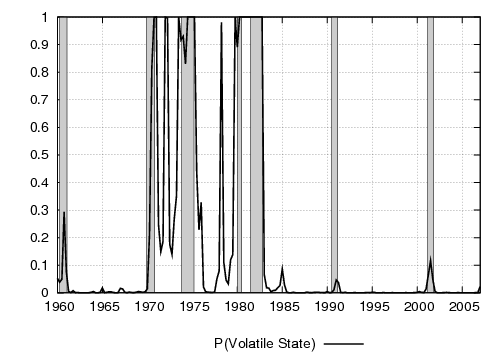
\includegraphics[scale=0.5]{results_re/states_sm.png} \\
\textbf{Dynamic Gain Learning} \\
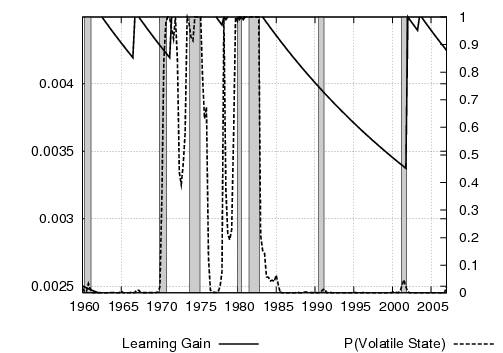
\includegraphics[scale=0.5]{results_dg8_wlsinit/states_sm.png} \\
\textbf{Constant Gain Learning} \\
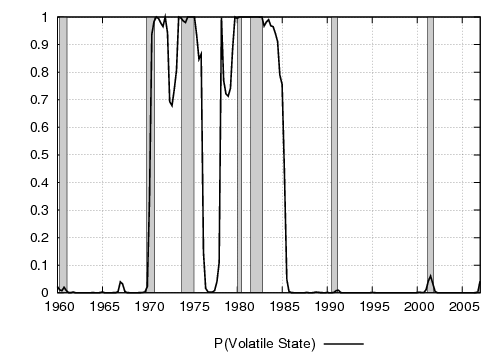
\includegraphics[scale=0.5]{results_cg_wlsinit/states_sm.png} 
\end{tabular}
\end{center}
\end{figure}

\begin{figure}[ht]
\caption{Smoothed Estimate of Natural Rate Shock}\label{fg:natrate}
\begin{center}
\begin{tabular}{c}
\textbf{Rational Expectations} \\  
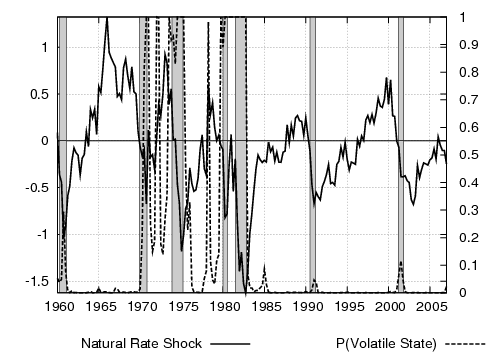
\includegraphics[scale=0.5]{results_re/natrate.png} \\
\textbf{Dynamic Gain Learning} \\
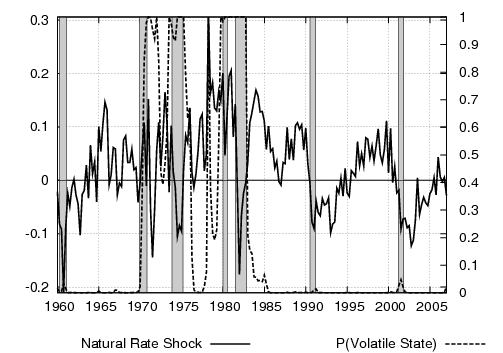
\includegraphics[scale=0.5]{results_dg8_wlsinit/natrate.png} \\
\textbf{Constant Gain Learning} \\
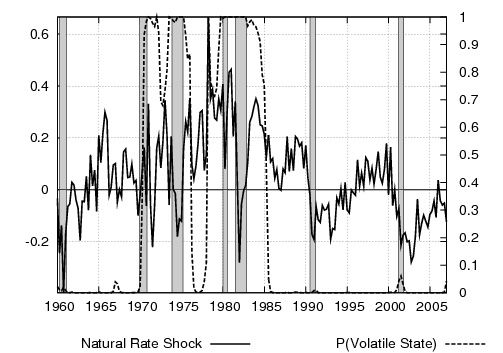
\includegraphics[scale=0.5]{results_cg_wlsinit/natrate.png} 
\end{tabular}
\end{center}
\end{figure}

\begin{figure}[ht]
\caption{Smoothed Estimate of Cost Push Shock}\label{fg:costpush}
\begin{center}
\begin{tabular}{c}
\textbf{Rational Expectations} \\  
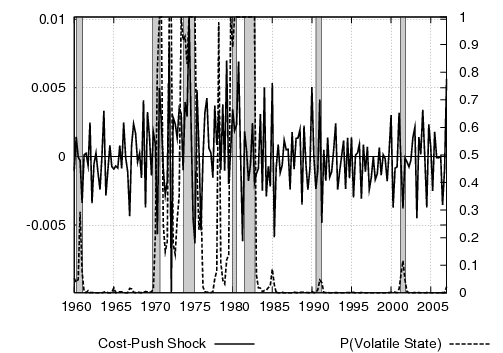
\includegraphics[scale=0.5]{results_re/costpush.png} \\
\textbf{Dynamic Gain Learning} \\
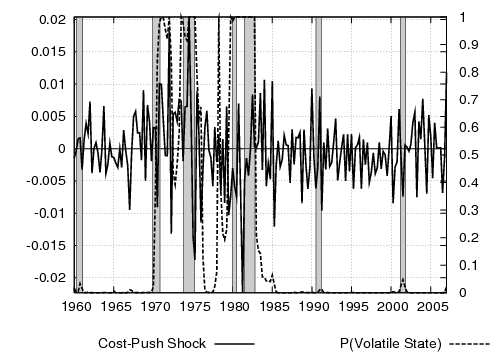
\includegraphics[scale=0.5]{results_dg8_wlsinit/costpush.png} \\
\textbf{Constant Gain Learning} \\
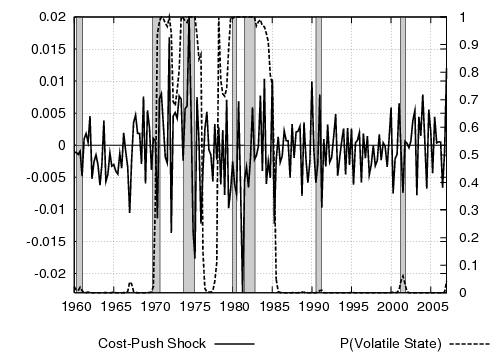
\includegraphics[scale=0.5]{results_cg_wlsinit/costpush.png} 
\end{tabular}
\end{center}
\end{figure}

\begin{figure}[ht]
\caption{Smoothed Estimate of Monetary Policy Shock}\label{fg:mpshock}
\begin{center}
\begin{tabular}{c}
\textbf{Rational Expectations} \\  
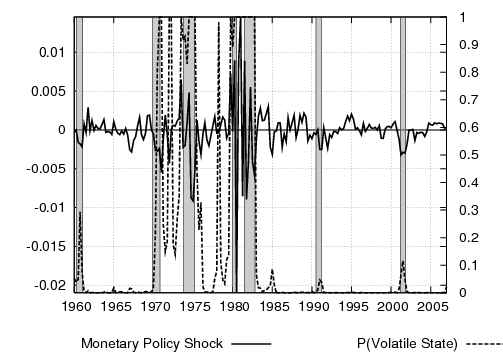
\includegraphics[scale=0.5]{results_re/mpshock.png} \\
\textbf{Dynamic Gain Learning} \\
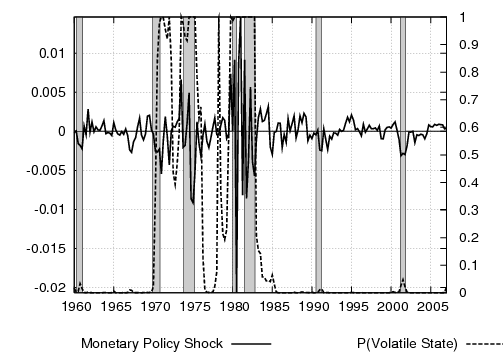
\includegraphics[scale=0.5]{results_dg8_wlsinit/mpshock.png} \\
\textbf{Constant Gain Learning} \\
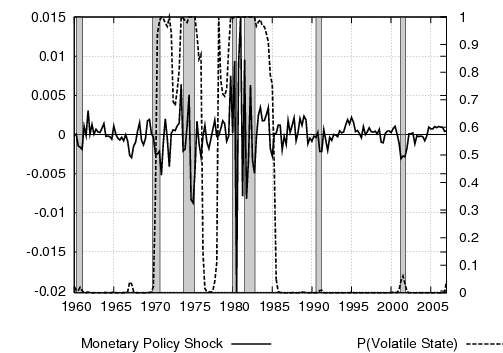
\includegraphics[scale=0.5]{results_cg_wlsinit/mpshock.png} 
\end{tabular}
\end{center}
\end{figure}

\begin{figure}[ht]
\caption{One Period Ahead Ouptut Forecast Error}\label{fg:outputerr}
\begin{center}
\begin{tabular}{c}
\textbf{Rational Expectations} \\  
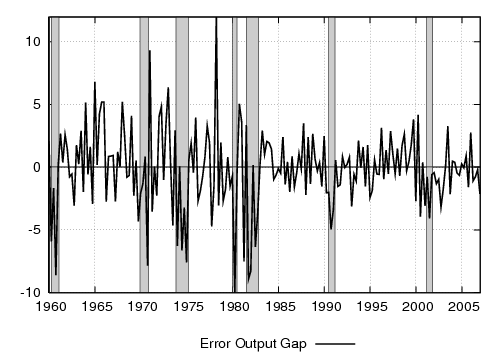
\includegraphics[scale=0.5]{results_re/output_err.png} \\
\textbf{Dynamic Gain Learning} \\
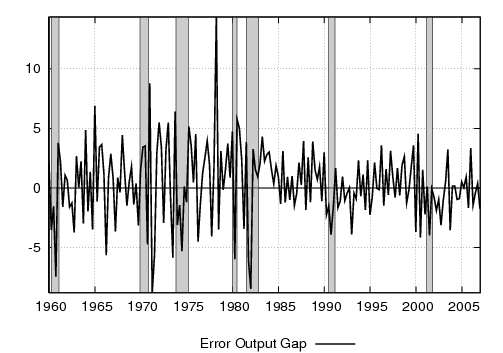
\includegraphics[scale=0.5]{results_dg8_wlsinit/output_err.png} \\
\textbf{Constant Gain Learning} \\
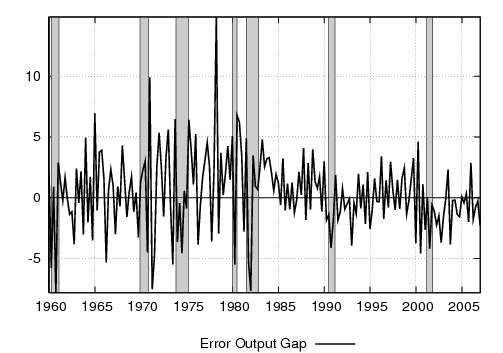
\includegraphics[scale=0.5]{results_cg_wlsinit/output_err.png} 
\end{tabular}
\end{center}
\end{figure}

\begin{figure}[ht]
\caption{One Period Ahead Inflation Forecast Error}\label{fg:inflationerr}
\begin{center}
\begin{tabular}{c}
\textbf{Rational Expectations} \\  
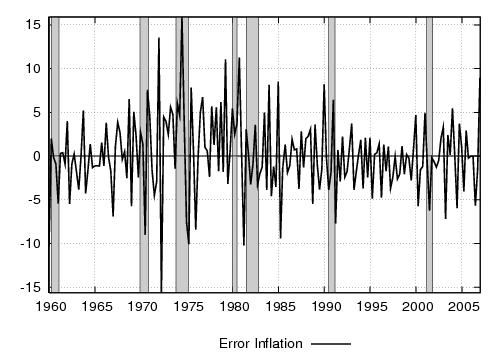
\includegraphics[scale=0.5]{results_re/inflation_err.png} \\
\textbf{Dynamic Gain Learning} \\
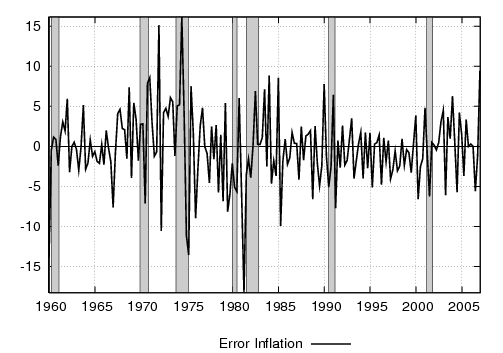
\includegraphics[scale=0.5]{results_dg8_wlsinit/inflation_err.png} \\
\textbf{Constant Gain Learning} \\
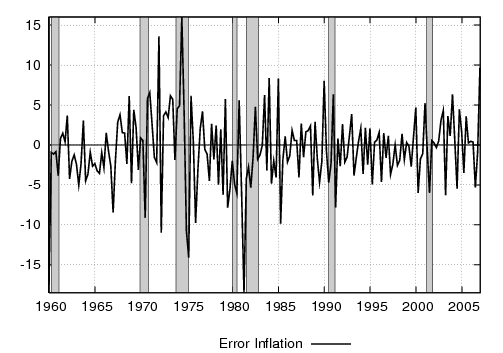
\includegraphics[scale=0.5]{results_cg_wlsinit/inflation_err.png} 
\end{tabular}
\end{center}
\end{figure}

\begin{figure}[ht]
\caption{One Period Ahead Federal Funds Rate Forecast Error}\label{fg:fedfundserr}
\begin{center}
\begin{tabular}{c}
\textbf{Rational Expectations} \\  
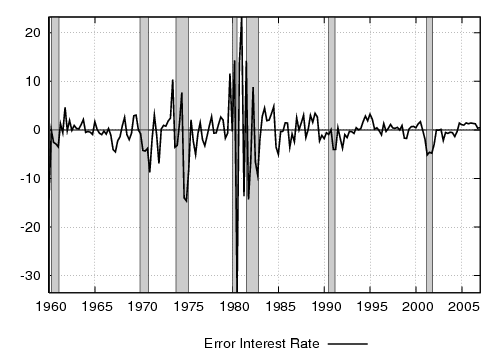
\includegraphics[scale=0.5]{results_re/fedfunds_err.png} \\
\textbf{Dynamic Gain Learning} \\
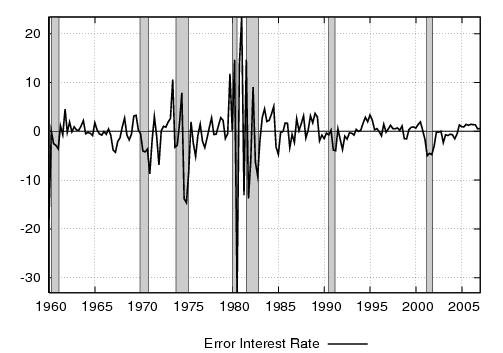
\includegraphics[scale=0.5]{results_dg8_wlsinit/fedfunds_err.png} \\
\textbf{Constant Gain Learning} \\
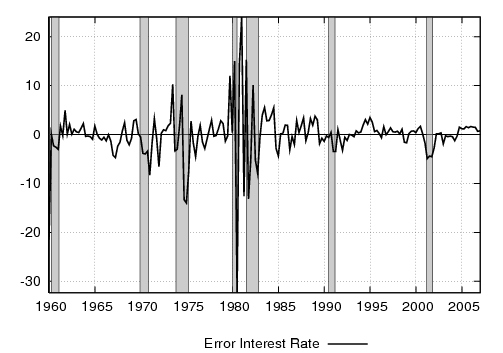
\includegraphics[scale=0.5]{results_cg_wlsinit/fedfunds_err.png} 
\end{tabular}
\end{center}
\end{figure}

\begin{figure}[ht]
\caption{Agents' Expectations}\label{fg:exp}
\begin{center}\hspace*{-0.65in}
\begin{tabular}{cc}
\multicolumn{2}{c}{\textbf{Dynamic Gain Learning}} \\
Output Gap & Inflation \\
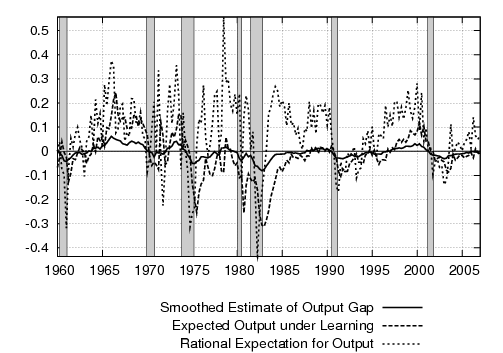
\includegraphics[scale=0.5]{results_dg8_wlsinit/output_expre.png} & 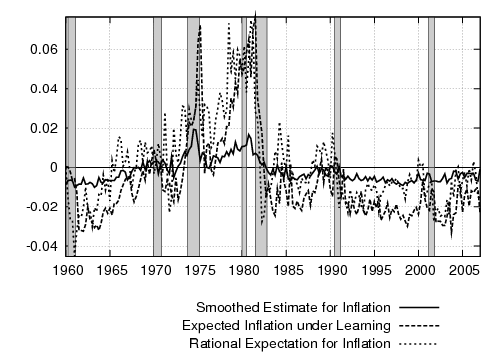
\includegraphics[scale=0.5]{results_dg8_wlsinit/inflation_expre.png} \\\\
\multicolumn{2}{c}{\textbf{Constant Gain Learning}} \\
Output Gap & Inflation \\
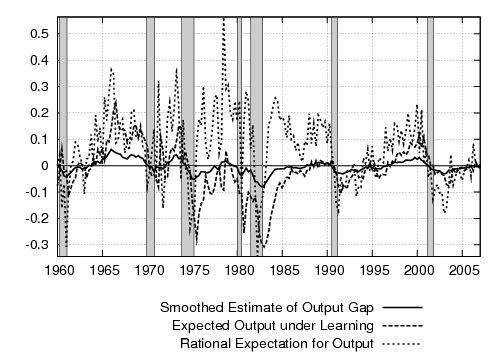
\includegraphics[scale=0.5]{results_cg_wlsinit/output_expre.png} & 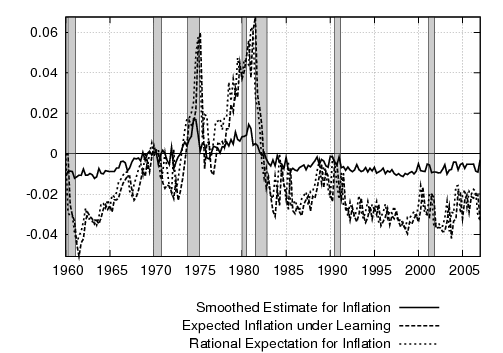
\includegraphics[scale=0.5]{results_cg_wlsinit/inflation_expre.png} \\
\end{tabular}
\end{center}
\end{figure}

\bibliographystyle{econometrica}
\bibliography{badluck}



\end{document}



